\documentclass[a4paper]{article}

%use the english line for english reports
%usepackage[english]{babel}
\usepackage[portuguese]{babel}
\usepackage[utf8]{inputenc}
\usepackage{indentfirst}
\usepackage{graphicx}
\usepackage{verbatim}


%Todas as figuras devem ser referidas no texto. %\ref{fig:codigoFigura}
%
%%Exemplo de código para inserção de figuras
%%\begin{figure}[h!]
%%\begin{center}
%%escolher entre uma das seguintes três linhas:
%%\includegraphics[height=20cm,width=15cm]{path relativo da imagem}
%%\includegraphics[scale=0.5]{path relativo da imagem}
%%\includegraphics{path relativo da imagem}
%%\caption{legenda da figura}
%%\label{fig:codigoFigura}
%%\end{center}
%%\end{figure}
%
%
%\textit{Para escrever em itálico}
%\textbf{Para escrever em negrito}
%Para escrever em letra normal
%``Para escrever texto entre aspas''
%
%Para fazer parágrafo, deixar uma linha em branco.
%
%Como fazer bullet points:
%\begin{itemize}
	%\item Item1
	%\item Item2
%\end{itemize}
%
%Como enumerar itens:
%\begin{enumerate}
	%\item Item 1
	%\item Item 2
%\end{enumerate}
%
%\begin{quote}``Isto é uma citação''\end{quote}

\begin{document}

\setlength{\textwidth}{16cm}
\setlength{\textheight}{22cm}

\title{\Huge\textbf{Morelli}\linebreak\linebreak\linebreak
\Large\textbf{Relatório Final}\linebreak\linebreak
\linebreak\linebreak

\includegraphics[scale=0.1]{feup-logo.png}\linebreak\linebreak
\linebreak\linebreak
\Large{Mestrado Integrado em Engenharia Informática e Computação} \linebreak\linebreak
\Large{Programação em Lógica}\linebreak
}

\author{\textbf{Grupo 3:}\\ Francisco Rodrigues - 201305627 \\ Marta Lopes - 201208067 \\\linebreak\linebreak \\
 \\ Faculdade de Engenharia da Universidade do Porto \\ Rua Roberto Frias, s\/n, 4200-465 Porto, Portugal \linebreak\linebreak\linebreak
\linebreak\linebreak\vspace{1cm}}
%\date{Junho de 2007}
\maketitle
\thispagestyle{empty}

%************************************************************************************************
%************************************************************************************************

\newpage

\section*{Resumo}

\par Este trabalho teve como finalidade consolidar todo o conhecimento que fomos adquirindo na cadeira de PLOG e aplica-lo para criar um produto final. 
\par Como grupo podemos dizer que cooperamos bastante e trabalhamos sempre lado-a-lado, tornando todo o desenvolvimento do jogo mais fácil e fluido. 
\par \textit{Prolog} é uma linguagem de programação que se enquadra do paradigma da Programação em Lógica Matemática o que a torna um pouco diferente das linguagens a que estávamos habituados o que tornou mais difícil a resolução de pequenos problemas que felizmente foram sendo resolvidos com recurso à consulta dos materiais fornecidos pelos professores. Com isso conseguimos alcançar um jogo final não tão completo como o que gostaríamos que fosse no inicio, mas estamos contentes com o que conseguimos desenvolver apesar de tudo. 
\newpage

\tableofcontents

%************************************************************************************************
%************************************************************************************************

%*************************************************************************************************
%************************************************************************************************

\newpage

%%%%%%%%%%%%%%%%%%%%%%%%%%
\section{Introdução}

\par Para este projeto tínhamos como objetivo desenvolver um jogo em linha de comandos, como tal, decidimos escolher o \textit{Morelli} porque achamos que seria um jogo apelativo e interessante para desenvolver. De inicio o jogo parecia bastante simples, mas à medida que foi sendo desenvolvido notamos um certo aumento da dificuldade, no entanto nunca deixamos de perceber a dinâmica de jogo.
\par Reparamos em certas semelhanças com o jogo \textit{Othello} e \textit{Ming Mang} mas no geral o jogo que nós desenvolvemos é muito mais abstracto que todos os outros jogos de tabuleiro que conhecemos. Este trabalho serviu então para avaliar todos os nossos conhecimentos nesta linguagem nova para nós, e desenvolvendo este jogo que é completamente diferente daquilo a que estamos habituados.
\par Este relatório encontra-se dividido nas seguintes secções: 
\begin{itemize}
	\item História e regras de jogo;
	\item Implementação da lógica de jogo;
	\item Descrição da interface;
	\item Conclusões sobre este projeto;
	\item Bibliografia;
	\item Anexos, como o código do projeto.
\end{itemize}	


%%%%%%%%%%%%%%%%%%%%%%%%%%
\section{Morelli}

\par \textit{Morelli} é um jogo de tabuleiro criado por \textit{Richar Moxham} em 2011. É jogado por apenas 2 jogadores num tabuleiro de 13x13 quadrados em faixas concêntricas. A faixa de fora será a maior, com 48 casas, terminando na casa central. 

\begin{itemize}
	\item O jogo começa com \textbf{24 peças pretas} e \textbf{24 peças brancas}, ambas reversíveis, posicionadas nos quadrados de fora, de forma diametralmente oposta. Para além disso cada jogador vai ter \textbf{uma torre da cor respectiva}, que não vai entrar no tabuleiro no inicio do jogo. 
\begin{figure}[h!]
\begin{center}
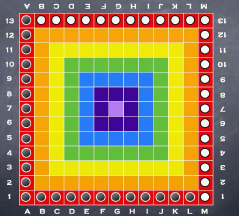
\includegraphics[scale=0.9]{fig1.png}
\caption{Inicio de Jogo}
\end{center}
\end{figure}

\item Cada jogador joga na sua vez, começando primeiro o jogador que tiver as peças da cor preta. Um \textbf{movimento legal} (Fig.2) consiste em mover a peça para um quadrado desocupado numa linha ortogonal ou diagonal desde que seja para uma faixa mais próxima do centro do que aquela em que se encontra no momento, não se podendo manter na mesma faixa ou voltar para trás (Fig.3).

\begin{figure}[h!]
\begin{center}
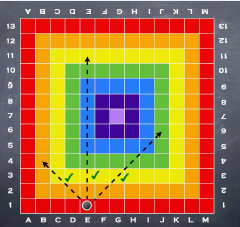
\includegraphics[scale=0.9]{fig2.png}
\caption{Movimento legal}
\end{center}
\end{figure}

\begin{figure}[h!]
\begin{center}
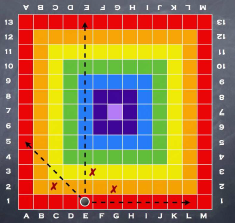
\includegraphics[scale=0.9]{fig3.png}
\caption{Movimento Ilegal}
\end{center}
\end{figure}

\newpage
\item Apenas será possivel passar pelo centro se este estiver vazio, não podendo parar nele. (Fig.4, Fig.5).

\begin{figure}[h!]
\begin{center}
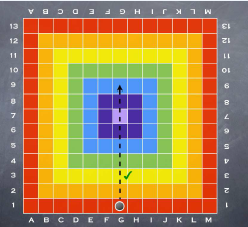
\includegraphics[scale=0.9]{center1.png}\linebreak\linebreak 
\caption{Movimento Legal}
\end{center}
\end{figure}

\begin{figure}[h!]
\begin{center}
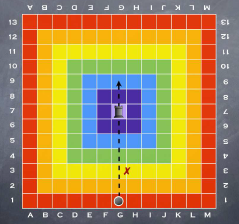
\includegraphics[scale=0.9]{center2.png}\linebreak\linebreak 
\caption{Movimento Ilegal}
\end{center}
\end{figure}


\newpage
\item A \textbf{captura do centro} é feita quando o jogador cria um quadrado de qualquer tamanho com as suas peças, centrado na célula central (Fig.4 e Fig.5). Quando o centro está capturado é colocada a torre da cor respectiva no centro do tabuleiro, removendo a torre adversária se se aplicar.


\begin{figure}[h!]
\begin{center}
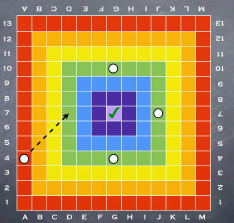
\includegraphics[scale=0.9]{fig4.png}
\caption{Captura do centro}
\end{center}
\end{figure}

\begin{figure}[h!]
\begin{center}
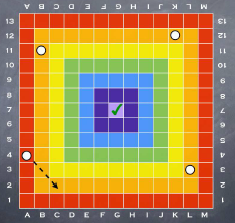
\includegraphics[scale=0.9]{fig41.png}
\caption{Captura do centro}
\end{center}
\end{figure}

\newpage
\item A cada movimento o jogador poderá \textbf{capturar uma peça adversária} quando conseguir rodea-la por duas peças da sua cor seja ortogonal ou diagonalmente (Fig.6). Uma peça capturada é revertida passando para a cor contrária. 

\begin{figure}[h!]
\begin{center}
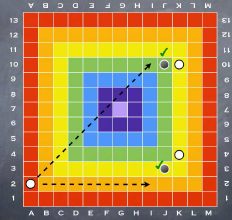
\includegraphics[scale=0.9]{fig5.png}
\caption{Captura de peça adversária}
\end{center}
\end{figure}


	\item O \textbf{vencedor} será o jogador que terá a sua torre no centro no final do jogo. O jogo acaba quando não existirem mais jogadas possíveis. Se o centro se mantiver sem nenhuma torre até ao final do jogo, é um empate. 

\end{itemize}



%%%%%%%%%%%%%%%%%%%%%%%%%%
\section{Lógica do Jogo}

\subsection{Representação do Estado do Jogo e Visualização do Tabuleiro} 
\par Sendo o tabuleiro de 13x13 o estado de jogo é representado numa matriz com esse tamanho, onde a partir dos predicados que obtêm e modificam o elemento vão substitui-lo para a visualização no tabuleiro. Cada elemento dessa lista será um espaço vazio, uma peça ou o centro vazio ou ocupado por uma torre. 
\par Para distinguir as peças dos dois jogadores, estas vão ter um valor diferente. As peças do jogador preto vão ter valor 1 e a sua torre o valor 4 e as peças do jogador branco vão ter valor 2 sendo que a sua torre terá o valor 5. O centro vazio terá o valor de -1 e o espaço vazio de 0. A visualização do tabuleiro é feita com o predicado \textbf{startDrawingBoard(\_, +BoardSize, -Board1)}. 
\par Na \textbf{visualização do tabuleiro}, as peças pretas serão um 'x' e a torre preta um 'X', já as peças brancas serão um 'o' e a sua torre um 'O'. O centro vazio será representado por um 'N'. 
\par A representação de vários estados do tabuleiro será então apresentada em baixo com a respectiva visualização do tabuleiro na consola. 

\begin{figure}
\begin{center}
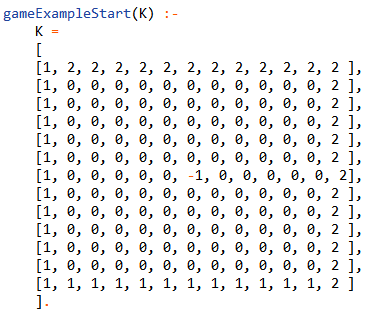
\includegraphics[scale=0.8]{gamestart.png}
\caption{Exemplo de um estado inicial do tabuleiro}
\end{center}
\end{figure}

\begin{figure}
\begin{center}
\hspace*{-0.1cm}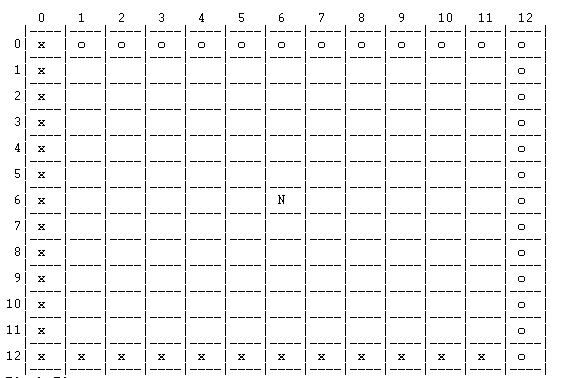
\includegraphics[scale=0.8]{gamestartboard.png}
\caption{Visualização de um estado inicial na consola}
\end{center}
\end{figure}


\begin{figure}
\begin{center}
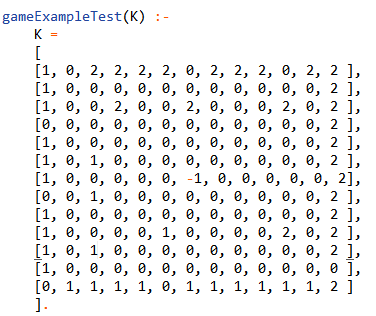
\includegraphics[scale=0.8]{gamemiddle.png}
\caption{Exemplo de um estado intermédio do tabuleiro}
\end{center}
\end{figure}

\begin{figure}
\begin{center}
\hspace*{-0.1cm}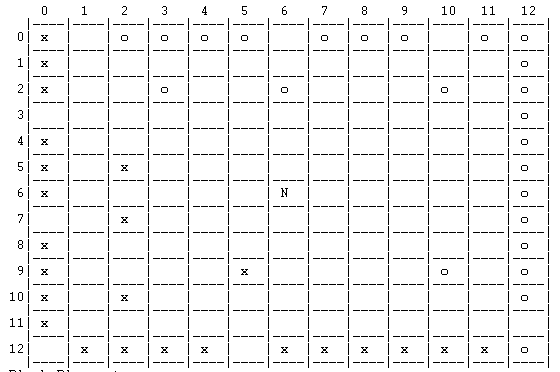
\includegraphics[scale=0.8]{gamemiddleboard.png}
\caption{Visualização de um estado intermédio na consola}
\end{center}
\end{figure}


\begin{figure}
\begin{center}
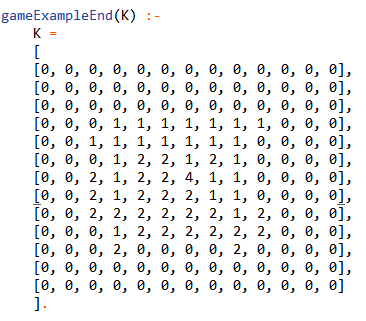
\includegraphics[scale=0.8]{gameend.png}
\caption{Exemplo de um estado final do tabuleiro}
\end{center}
\end{figure}

\begin{figure}
\begin{center}
\hspace*{-0.1cm}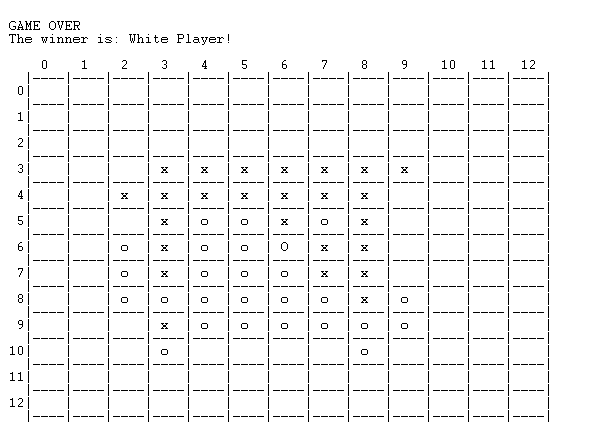
\includegraphics[scale=0.8]{gameendboard.png}
\caption{Visualização de um estado final na consola}
\end{center}
\end{figure}

\newpage
\subsection{Lista de Jogadas Válidas}

\par A lista de listas jogadas válidas vai ser obtida a partir do predicado \textbf{validMoves(0,0,13, +Piece, +Board, -ListOfMoves)}. A lista de cada jogada vai conter no inicio as coordenadas de origem da peça pretendida e de seguida todas as coordenadas possiveis de destino para essa peça, por exemplo: 
\par [ [0, 0, [1,1], [2,2], [3,3], [4,4], [5,5], [7,7], [8,8], [9,9], [10,10], [11,11]]. 
\begin{figure}[h!]

\hspace*{-0.5cm}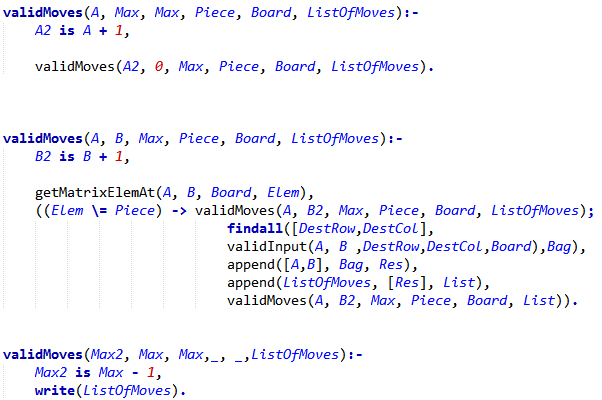
\includegraphics[scale=0.85]{listajogadas.png}
\caption{Código para gerar a lista de jogadas válidas}

\end{figure}


\subsection{Execução de Jogadas}


\par A cada jogada, é pedido ao jogador as coordenadas da peça que deseja mover e as coordenadas de destino da respectiva peça. Ao longo deste processo, vão ser feitas as seguintes verificações: 
\begin{enumerate}
	\item \textbf{getPieceCoords(+Board, +Player,+CurrRow, +CurrCol)} vai verificar se as coordenadas de origem correspondem à peça do jogador respectivo. 
	\item \textbf{getDestCoords(+Board, +Player, +CurrRow, +CurrCol, +DestRow, +DestCol)} vai ter os predicados de verificação e execução do \textit{move}
	\subitem 2.1. O predicado de verificação, \textbf{validInput(+CurrRow, +CurrCol, +DestRow, +DestCol, +Board)}, vai fazer todas as verificações de acordo com as regras para saber se o movimento é legal ou não. Se for legal a matriz vai ser alterada. 
	\subitem 2.2. Após a alteração da matriz vão ser usados predicados para verificar capturas (\textbf{checkCapture(+DestRow, +DestCol, +Piece,+ Board2, -Board3)}) e a captura do centro (\textbf{checkCenter(+DestRow, \linebreak +DestCol,+Piece, +Board3, -Board4)}). A captura do centro é verificada não só para a peça que foi movimentada, mas também para as peças que possam ser capturadas na sequência da jogada. 
\end{enumerate}

Depois de todas as verificações e alterações na matriz de jogo, é chamado o predicado \textbf{switchPlayer(-NextPlayer, +Player)} que vai alternar os jogadores no fim de cada jogada.

\subsection{Final de Jogo}
Quando o predicado de jogo é chamado, é sempre verificado o final de jogo com o predicado \textbf{checkEnd(+Board, 1, 1, 13, +Piece)}, se não houver mais movimentos possiveis para o jogador que está a jogar este predicado chama o predicado \textbf{gameOver(+Board)} que vai terminar o jogo dizendo o vencedor ou, se for o caso, devolver um empate e regressar ao menu inicial.

\section{Jogada do Computador}

\par Devido à falta de tempo apenas nos foi possivel implementar o \textbf{random bot}. É feito no predicado \textbf{getRandomPlay(+Board, +ListOfMoves,+ Player)} que antes já passou pelo predicado \textbf{validMoves} que vai gerar as jogadas possiveis para um dado jogador. 
\par O \textit{bot} vai escolher da lista de listas de jogadas, uma lista aleatória, obtendo nas primeiras duas posições a posição original da peça. De seguida, vai escolher da lista uma jogada possível e vai implementa-la. As verificações de captura de peças adversárias, de centro e de fim de jogo também são implementadas neste caso. 
%%%%%%%%%%%%%%%%%%%%%%%%%%

\newpage
\section{Interface com o Utilizador}

A interface da linha de comandos foi feita para ser simples de perceber e para facilitar a experiência de jogo. Os menus de navegação estão identificados e para navegar entre eles é necessário escolher o número correspondente e pressionar \textit{Enter}. O jogador para além do menu de jogo, poderá aceder a um pequeno resumo das regras, e um \textit{About}.

\begin{figure}[h!]
\begin{center}
\hspace*{-0.5cm}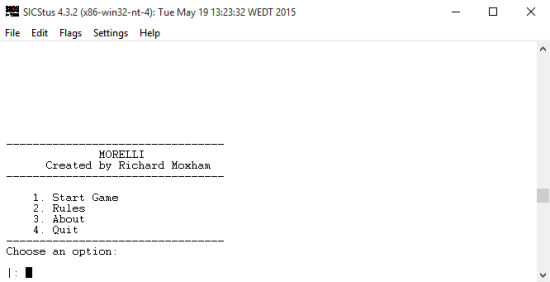
\includegraphics[scale=0.9]{menu1.png}
\caption{Menu inicial}
\end{center}
\end{figure}

\begin{figure}[h!]
\begin{center}
\hspace*{-0.5cm}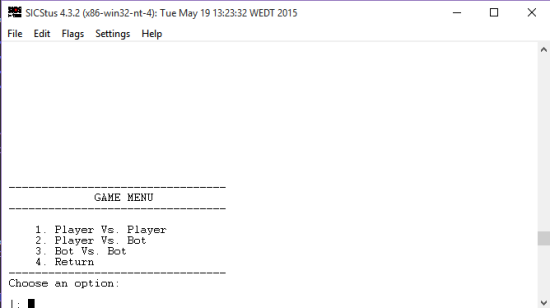
\includegraphics[scale=0.9]{menu2.png}
\caption{Menu de Jogo}
\end{center}
\end{figure}

\newpage
\par Durante o jogo a linha de comandos é limpa, é exibida uma mensagem para o jogador respectivo iniciar a jogada, e o estado atual do tabuleiro é imprimido na consola. É então solicitado ao jogador as coordenadas da peça que quer movimentar e as coordenadas de destino. 
\par Para a inserção de coordenadas o jogador terá que inserir primeiro a \textit{Row} e de seguida a \textit{Column}. Quando o jogador tenta jogar com uma peça que não seja a dele, ou mover a sua peça para um destino inválido, são exibidas mensagens de erro e o jogador terá de recomeçar a inserção das coordenadas de origem e destino. 

\begin{figure}[h!]
\begin{center}
\hspace*{-0.5cm}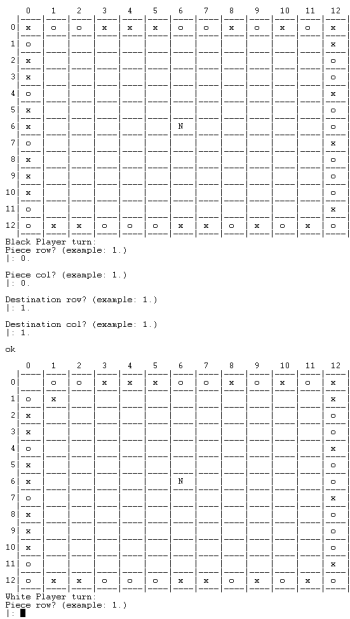
\includegraphics[scale=1]{game1.png}
\caption{Realização de uma jogada}
\end{center}
\end{figure}

\begin{figure}
\begin{center}
\hspace*{-0.5cm}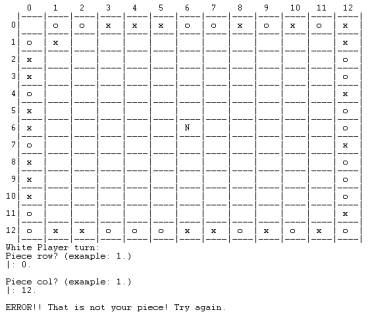
\includegraphics[scale=1]{game2.png}
\caption{Exemplo de uma seleção de peça inválida}
\end{center}
\end{figure}

\begin{figure}
\begin{center}
\hspace*{-0.5cm}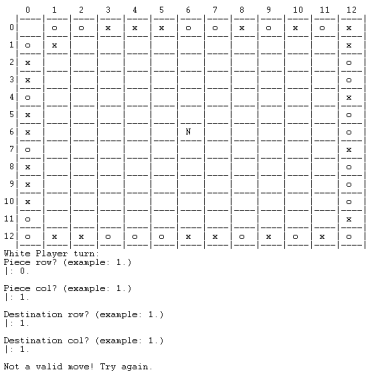
\includegraphics[scale=1]{game3.png}
\caption{Exemplo de uma escolha de coordenadas de destino inválidas}
\end{center}
\end{figure}



%%%%%%%%%%%%%%%%%%%%%%%%%%
\newpage
\section{Conclusões}
Para a realização do Morelli foi dispendido bastante tempo mas achamos que o resultado final foi positivo e conseguimos com este projecto adquirir bastantes conhecimentos. Apesar de acharmos que o tempo para a entrega final poderia ter sido maior, foi possivel concluir uma grande parte do projecto. 
\par As dificuldades que fomos encontrando ao longo do desenvolvimento foram superadas, apesar de que a implementação do \textit{bot} não foi implementada totalmente e também poderiamos ter melhorado algumas partes do código para não ficar tão extenso. 



\clearpage
\addcontentsline{toc}{section}{Bibliografia}
\renewcommand\refname{Bibliografia}
\bibliographystyle{plain}
\bibliography{myrefs}
\par [1] "Morelli." BoardGameGeeks. N.p., 2011. Web. 2015.
\par [2] "Morelli at Boardspace.net"  Boardspace.net. N.p., 2011. Web. 2015.

\newpage
\appendix
\section{Pasta \textit{code}}
O código \textit{Prolog} do projeto encontra-se na pasta \textit{code} que está anexada junto deste relatório.

\end{document}
